
\section{Newton Polynomische Interpolation}
\subsection{Collocation}
Collocation = Alle Messpunkte werden von angenäherter Funktion (z.B. Polynom) getroffen.

\subsection{Aitken-Neville Rekursionsformel}
Sich an den Messpunkten $x_1,\ldots, x_{n-1}$ überlappende polynomiale Interpolationsfunktionen 
$f_1=p_{0,1,\ldots,n-1}$, $f_2=p_{1,\ldots,n}$ können zusammengefasst werden. 

\begin{minipage}{9.5cm}
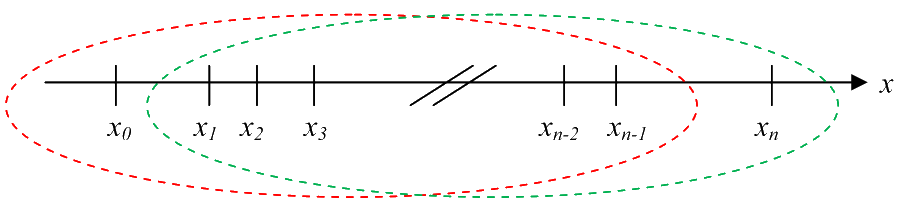
\includegraphics[width=\textwidth]{bilder/aitkenNevilleIdee}
\end{minipage}
\hfill
\begin{minipage}{9.5cm}
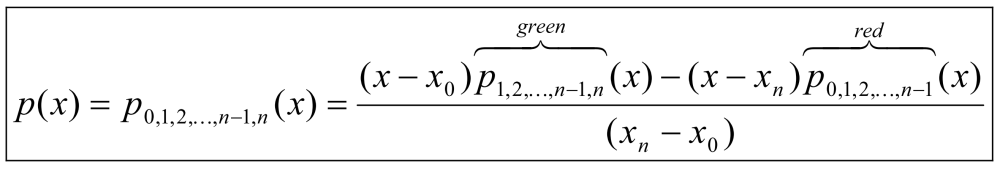
\includegraphics[width=\textwidth]{bilder/aitkenNevilleFormel}
\end{minipage}

\subsection{Newton Polynome}
\textbf{Eigenschaften}
\begin{liste}
	\item[\textbf{+}] Eingebettet (Wenn ein Messwert dazukommt muss nicht alles neu berechnet werden)
	\item[\textbf{+}] Eine einzige Formel
	\item[\textbf{+}] Praktisch: Messungen sind gleichverteilt.
	\item[$\mathbf{-}$] Runge-Phänomen (Schwingungen am Rand)
	\item[$\mathbf{-}$] Aufwändig zum rechnen
\end{liste}
\begin{minipage}[t]{7.5cm}
	\begin{align}
		y_0 &= a_0\cdot \pi_0 \nonumber\\
		&\quad \downarrow\nonumber\\
		y_1 &= a_0\cdot \pi_0 +a_1\cdot\pi_1 \nonumber\\
		&\quad \downarrow \hspace{1.2cm}\downarrow\nonumber\\
		y_2 &= a_0\cdot \pi_0 +a_1\cdot\pi_1  +a_2\cdot\pi_2  \nonumber\\
		&\vdots\hspace{0.3cm}\downarrow \hspace{1.5cm}\searrow\hspace{1.5cm}\searrow\nonumber\\
		y_n &= a_0\cdot \pi_0(x_n) +a_1\cdot\pi_1(x_n)  +a_2\cdot\pi_2(x_n)+\ldots+ a_n\pi_n(x_n) \nonumber
	\end{align}	
	Annäherung an ``Messreihe'' mit Polynomen: $$y(x)\approx p(x) = a_0 \pi_0(x) + a_1 \pi_1(x) + \ldots+ a_{n} \pi_{n}(x)$$
\end{minipage}
\hfill
\begin{minipage}[t]{11.5cm}
	\begin{align}
		\pi_0 &= 1 \nonumber\\
		\pi_1 &= (x-x_0) \nonumber\\
		\pi_2 &= (x-x_0)(x-x_1) \nonumber\\
		&\vdots \nonumber\\
		\pi_n &= (x-x_0)(x-x_1)\ldots(x-x_{n-1}) \nonumber\\
		\pi_{n+1} &= (x-x_0)(x-x_1)\cdots(x-x_{n-1})(x-x_n) \nonumber
	\end{align}	
\end{minipage}
\subsection{Dividierte Differenzen}
Elegantere und schnellere Auflösung der Newton Polynome.
$$y(x_\mathbf{0}, x_1, \ldots x_\mathbf{k-1}) = \frac{y(x_\mathbf{1},x_2,\ldots x_\mathbf{k})-y(x_\mathbf{0},x_1,\ldots x_{\mathbf{k-1}})}{(x_k-x_0)} \quad (k=0,1,\ldots,n)$$
$$a(x_\mathbf{0},\ldots,x_\mathbf{n})=\frac{a(x_\mathbf{1},\ldots,x_\mathbf{n})-a(x_\mathbf{0},\ldots,x_{\mathbf{n-1}})}{x_n-x_0}$$
\begin{tabular}{ll}
$k=0$ &$y(x_0)$ \\[0.2cm]
$k=1$ &$\frac{y(x_1)-y(x_0)}{(x_1-x_0)}$\\[0.2cm]
$k=2$ &$\frac{y(x_1,x_2)-y(x_0,x_1)}{(x_2-x_0)}$\\[0.2cm]
$k=3$ &$\frac{y(x_1,x_2,x_3)-y(x_0,x_1,x_2)}{(x_3-x_0)}$\\
\end{tabular}\\
\\

\textbf{Beispiel:}\\
\begin{minipage}[c]{6.0cm}
	\begin{tabular}{|c||c|llll|}
	\hline
			&$x_k$	&\multicolumn{4}{l|}{$y_k$}\\
	\hline
	$x_0$	&$0$	&\kreisS{$1$}{$a_0$}&			&			&\\
		 	&		&			&\kreisS{$0$}{$a_1$}&			&\\
	$x_1$	&$1$	&$1$		&			&\kreisM{$\frac 12$}{$a_2$}&\\
			&		&			&$1$		&			&\kreisB{$-\frac{1}{12}$}{$a_3$}\\
	$x_2$	&$2$	&$2$		&			&$\frac 16$&\\
			&		&			&$\frac{3}{2}$		&			&\\
	$x_3$	&$4$	&$5$		&			&			&\\
	\hline
	\end{tabular}
\end{minipage}
\hfill
\begin{minipage}[c]{13cm}
	\begin{alignat}{4}
		y(x)\approx p(x)&=a_0\cdot \pi_0(x) &&+a_1\cdot\pi_1(x)  &&+a_2\cdot\pi_2(x)&&+ a_3\pi_n(x)\nonumber\\[0.3cm]
		&=1\cdot \pi_0(x) &&+0\cdot\pi_1(x)  &&+\frac 12\cdot\pi_2(x)&&- \frac 1{12}\pi_n(x)\nonumber %\\[0.3cm]
		%&=1&&&&+\frac 12 (x-x_0)(x-x_1) &&-\frac 1{12} (x-x_0)(x-x_1)(x-x_2)\nonumber
	\end{alignat}
	\begin{alignat}{3}
	y(x)\approx p(x)&=1&&+\frac 12(x-x_0)(x-x_1)&&-\frac 1{12} (x-x_0)(x-x_1)(x-x_2)\nonumber\\[0.3cm]
	&=1&&+\frac 12(x-0)(x-1)&&-\frac 1{12} (x-0)(x-1)(x-2)\nonumber
	\end{alignat}
\end{minipage}


\subsection{Collocation Fehlerformel}
$$y(x)-p(x) = \frac{f^{(n+1)}(\xi)}{(n+1)!} (x-x_0)(x-x_1)\ldots(x-x_{n-1})(x-x_n) = \frac{f^{(n+1)}(\xi)}{(n+1)!}\pi_{n+1}(x) \quad \xi \in (\min(x_i), \max(x_i))$$

\subsection{Runge Phänomen und Chebyshev Argumente}
Runge Phänomen: Potenzielle Oszillationen an den Definitionsrändern von Polynom-Collocations.\\
Chebyshev-Argumente: Anpassung der Messpunkte durch andere Verteilung (nicht mehr gleichverteilte $x_k$, sondern am Einheitskreis gleichverteilte)
$x_k = \cos({\frac{2k+1}{2(n+1)}\pi), (k=0,1,\ldots,n)})$
ergibt maximale Amplitude $\max_{-1\leq x\leq 1}|\pi_{n+1}(x)| = \frac{1}{2^n}$. Mit affiner Formel von Einheitsinterval $[-1,1]$ zu $[a,b]$: $x \rightarrow a+\frac{b-a}{2}(x+1)$
\begin{center}
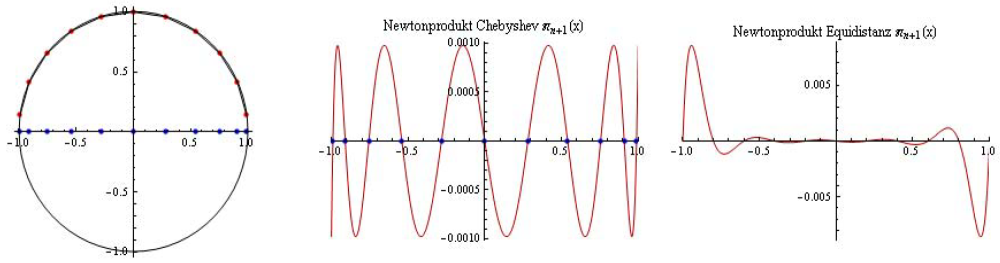
\includegraphics[width=14cm]{bilder/TschbyNewtonVergleich.png}
\end{center}

\textbf{Eigenschaften}
\begin{liste}
  \item[\textbf{+}] Kein Runge-Phänomen (Schwingungen am Rand)
  \item[\textbf{+}] Eine einzige Formel
  \item[$\mathbf{-}$] "`Nicht eingebettet"' (neue Messungen bedeutet, neue Polynomberechnung!)
  \item[$\mathbf{-}$] Praktisch: Messungen sind oft nur gleichverteilt möglich (Randauflösung beschränkt)
  \item[$\mathbf{-}$] Der Bereich der Interpolation ist fixiert
\end{liste}

\subsection{Gleichverteilte Argumente}


\begin{minipage}[c]{11.0cm}
	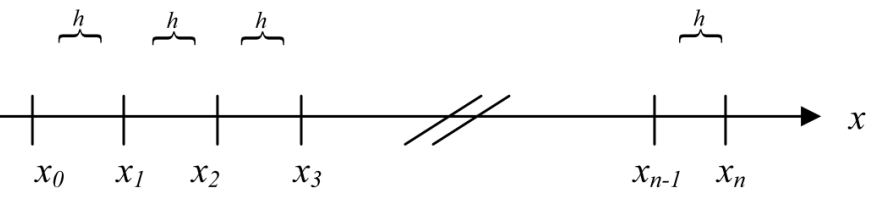
\includegraphics[width=\textwidth]{bilder/gleichvArgum.png}	
\end{minipage}
\begin{minipage}[c]{6.0cm}
	$$x_k=x_0+k h\qquad k=0,1,2,\ldots n$$
	$$y(x_0,x_1,\ldots,x_k)=\frac{\Delta^k y_0}{h^k k!}$$
\end{minipage}
\hfill\\

$$p(x)=y_0+\frac{\Delta^1 y_0}{h^1 1!}\pi_1(x)+\frac{\Delta^2 y_0}{h^2 2!}\pi_2(x)+\ldots+\frac{\Delta^n y_0}{h^n n!}\pi_n(x)=\sum\limits_{k=0}^{n}{\frac{\Delta^k y_0}{h^k k!}\pi_k(x)}$$

\begin{tabular}{|c|ll|}
\hline
y		& $\Delta^1$	& $\Delta^2$\\
\hline
$y_0$	&&\\
$y_1$	& $y_1-y_0=\Delta^1y_0$&\\
$y_2$	& $y_2-y_1=\Delta^1y_1$	& $\Delta^1 y_1 - \Delta^1 y_0 = y_2 - 2y_1 +y_0=\Delta^2y_0 \text{(wenn gleichverteilt)}$\\
\hline
\end{tabular}

\subsection{Taylor Reihe}
$$f(x)=\underset{\text{Taylor Polynom p(x)}}{\underbrace{y_0+\frac{y'(x_0)}{1!}(x-x_0)+\frac{y''(x_0)}{2!}(x-x_0)^2+\ldots+\frac{y^{(n)}(x_0)}{n!}(x-x_0)^n}}+\underset{\text{Lagrange Fehlerterm}}{\underbrace{\frac{y^{(n+1)}(\xi)}{(n+1)!}(x-x_0)^{n+1}}}$$
